\chapter{Latex-Bausteine}\label{Stile}

Der Text wird in bis zu drei Ebenen gegliedert:

\begin{enumerate}
  \item Kapitel ( \verb \chapter{Kapitel} ), \index{Kapitel}
  \item Unterkapitel  (  \\section{Abschnitt} ) und
  \item Unterunterkapitel  ( \\subsection{Unterabschnitte} ).
\end{enumerate}

\section{Abschnitt}\index{Abschnitt}
Text der Gliederungsebene 2.


\subsection{Unterabschnitt} \index{Unterabschnitt}
Text der Gliederungsebene 3. Text Text Text Text Text Text Text Text Text Text Text Text Text Text Text. Beispiel für Quelltext\index{Quelltext} \\[2 ex]
\noindent
\begin{minipage}{1.0\textwidth} \small
	\begin{lstlisting}
		Prozess 1:
	
		Acquire();
			a := 1;
		Release();
		...
		Acquire();
		if(b == 0)
		{					
			c := 3;
			d := a;
		}				
		Release();
	\end{lstlisting}
\end{minipage}

\vspace{2cm}
\noindent
\begin{minipage}{1.0\textwidth} \small
	\begin{lstlisting}
		Prozess 2:
	
		Acquire();
			b := 1;
		Release();
		...
		Acquire();
		if(a == 0)
		{					
			c := 5;
			d := b;
		}				
		Release();
	\end{lstlisting}
\end{minipage}
\vskip 1em

Größere Code-Fragmente sollten im Anhang eingefügt werden.

\section{Abbildungen und Tabellen}

Abbildungen\index{Abbildung} und Tabellen\index{Tabelle} werden zentriert eingefügt. Grundsätzlich sollen sie erst dann erscheinen, nach dem sie im Text angesprochen wurden (siehe Abb. \ref{a1}). Abbildungen und Tabellen (siehe Tabelle \ref{t1}) können im (fließenden) Text ( here ), am Seitenanfang (\verb top ), am Seitenende (\verb bottom ) oder auch gesammelt auf einer nachfolgenden Seite (\verb page ) oder auch ganz am Ende der Ausarbeitung erscheinen. Letzteres sollte man nur dann wählen, wenn die Bilder günstig zusammen zu betrachten sind und die Ausarbeitung nicht zu lang ist ($< 20$ Seiten).

\begin{figure} %[hbtp] %Optionen für layout
	\centering
	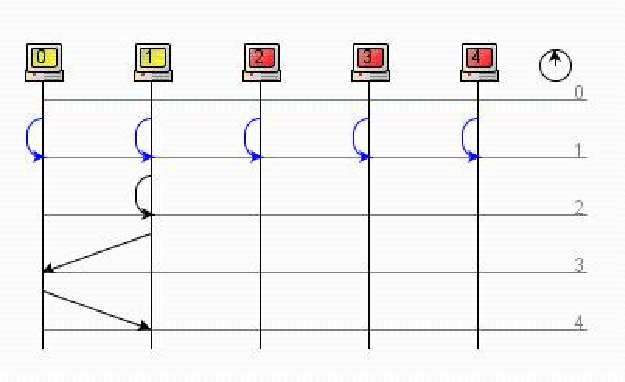
\includegraphics{images/p1ReadSeq.pdf}
	\caption{Bezeichnung der Abbildung}
	\label{a1}
\end{figure}

\begin{table} %[hbtp]
	\centering
	\begin{tabular}{l | l l l l} %Definiert Spalten der Tabelle
		\textbf{Prozesse} & \textbf{Zeit} $\rightarrow$ \\
		\hline
			$P_{1}$ & $W(x)1$ \\
			$P_{2}$ & & $W(x)2$ \\
			$P_{3}$ & & $R(x)2$ & & $R(x)1$\\
			$P_{4}$ & & & $R(x)2$ & $R(x)1$\\
	\end{tabular}
	\caption{Bezeichnung der Tabelle}
	\label{t1}
\end{table}


\section{Mathematische Formel}\index{Formel}
Mathematische Formeln bzw. Formulierungen können sowohl im laufenden Text (z.B. $y=x^2$) oder abgesetzt und zentriert im Text erscheinen. Gleichungen sollten für Referenzierungen nummeriert werden (siehe Formel \ref{gl-1}).
\begin{equation}\label{gl-1}
	e_{i}=\sum _{i=1}^{n}w_{i}x_{i}
\end{equation}

Entscheidungsformel:

\begin{equation}
	\psi(t)=\left\{
	\begin{array}{ccc}
		1 &  \qquad 0 <= t < \frac{1}{2} \\
		-1 &  \qquad \frac{1}{2} <= t <1 \\
		0 & \qquad sonst
	\end{array} \right.
\end{equation}


Matrix:\index{Matrix}
\begin{equation}
	A = \left(
	\begin{array}{llll}
		a_{11} & a_{12} & \ldots & a_{1n} \\
		a_{21} & a_{22} & \ldots & a_{2n} \\
		\vdots & \vdots & \ddots & \vdots \\
		a_{n1} & a_{n2} & \ldots & a_{nn} \\
	\end{array}
	\right)
\end{equation}

Vektor:\index{Vektor} 

\begin{equation}
	\overline{a} = \left(
	\begin{array}{c}
		a_{1}\\
		a_{2}\\
		\vdots\\
		a_{n}\\
	\end{array}
	\right)
\end{equation}

\section{Sätze, Lemmas und Definitionen}\index{Satz}\index{Lemma}\index{Definition}

Sätze, Lemmas, Definitionen, Beweise,\index{Beweis} Beispiele\index{Beispiel} können in speziell dafür vorgesehenen Umgebungen erstellt werden.

\begin{definition}(Optimierungsproblem)
	Ein \emph{Optimierungsproblem} $\mathcal{P}$ ist festgelegt durch ein Tupel
	$(I_\mathcal{P}, sol_\mathcal{P}, m_\mathcal{P}, goal)$ wobei gilt

	\begin{enumerate}
		\item $I_\mathcal{P}$ ist die Menge der Instanzen,
		\item $sol_\mathcal{P} : I_\mathcal{P} \longmapsto \mathbb{P}(S_\mathcal{P})$ ist eine Funktion, die jeder Instanz $x \in I_\mathcal{P}$ eine Menge zulässiger Lösungen zuweist,
		\item $m_\mathcal{P} : I_\mathcal{P} \times S_\mathcal{P} \longmapsto \mathbb{N}$ ist eine Funktion, die jedem Paar $(x,y(x))$ mit $x \in I_\mathcal{P}$ und $y(x) \in sol_\mathcal{P}(x)$ eine 	Zahl $m_\mathcal{P}(x,y(x)) \in \mathbb{N}$ zuordnet (= Maß für die Lösung $y(x)$ der Instanz $x$), und
		\item $goal \in \{min,max\}$.
	\end{enumerate}
\end{definition}

\begin{example} 
	MINIMUM TRAVELING SALESMAN (MIN-TSP)
	\begin{itemize}
		\item $I_{MIN-TSP} =_{def}$ s.o., ebenso $S_{MIN-TSP}$
		\item $sol_{MIN-TSP}(m,D) =_{def} S_{MIN-TSP} \cap \mathbb{N}^m$ 
		\item $m_{MIN-TSP}((m,D),(c_1, \ldots , c_m)) =_{def} \sum_{i=1}^{m-1} D(c_i, c_{i+1}) + D(c_m,c_1)$ 
		\item $goal_{MIN-TSP} =_{def} min$
	\end{itemize}
	\begin{flushright}
	$\qed$
	\end{flushright}
\end{example}

\begin{theorem} 
	Sei $\mathcal{P}$ ein \textbf{NP}-hartes Optimierungsproblem.
	Wenn $\mathcal{P} \in$ \textbf{PO}, dann ist \textbf{P} = \textbf{NP}.
\end{theorem}

\begin{proof} 
	Um zu zeigen, dass \textbf{P} = \textbf{NP} gilt, genügt es wegen Satz A.30 zu zeigen, dass ein einziges \textbf{NP}-vollständiges Problem in \textbf{P} liegt. Sei also $\mathcal{P}'$ ein beliebiges \textbf{NP}-vollständiges Problem.

	Weil $\mathcal{P}$ nach Voraussetzung \textbf{NP}-hart ist, gilt insbesondere $\mathcal{P}' \leq_T \mathcal{P}_C$. Sei $R$ der zugehörige Polynomialzeit-Algorithmus dieser Turing-Reduktion. Weiter ist $\mathcal{P} \in$ \textbf{PO} vorausgesetzt, etwa vermöge eines Polynomialzeit-Algorithmus $A$. Aus den beiden Polynomialzeit-Algorithmen $R$ und $A$ erhält man nun leicht einen effizienten Algorithmus für $\mathcal{P}'$: Ersetzt man in $R$ das Orakel durch $A$, ergibt dies insgesamt eine polynomielle Laufzeit. 
	\begin{flushright}
		$\qed$
	\end{flushright}
\end{proof}

\begin{lemma} 
	Aus \textbf{PO} $=$ \textbf{NPO} folgt \textbf{P} $=$ \textbf{NP}.
\end{lemma}

\begin{proof} 
	Es genügt zu zeigen, dass unter der angegeben Voraussetzung KNAPSACK $\in$ \textbf{P} ist.

	Nach Voraussetung ist MAXIMUM KNAPSACK $\in$ \textbf{PO}, d.h. die Berechnung von $m^*(x)$ für jede Instanz $x$ ist in Polynomialzeit möglich. Um KNAPSACK bei Eingabe $(x,k)$ zu entscheiden, müssen wir nur noch $m^*(x) \geq k$ prüfen. Ist das der Fall, geben wir $1$, sonst $0$ aus. Dies bleibt insgesamt ein Polynomialzeit-Algorithmus. 
	\begin{flushright}
		$\qed$
	\end{flushright}
\end{proof}

\section{Fußnoten}

In einer Fußnote können ergänzende Informationen\footnote{Informationen die für die Arbeit zweitrangig sind, jedoch für den Leser interessant sein könnten.} angegeben werden. Außerdem kann eine Fußnote auch Links enthalten. Wird in der Arbeit eine Software (zum Beispiel Java-API\footnote{\url{http://java.sun.com/}}) eingesetzt, so kann die Quelle, die diese Software zur Verfügung stellt in der Fußnote angegeben werden.

\section{Literaturverweise}\index{Literatur}
Alle benutzte Literatur wird im Literaturverzeichnis angegeben\footnote{Dazu wird ein sogennanter bib-File, literatur.bib verwendet.}. Alle angegebene Literatur sollte mindestens einmal im Text referenziert werden\cite{Coulouris:02}.
